\let\lesson\undefined
\newcommand{\lesson}{\phantomlesson{Bài 7.}}
\section{Bài tập trắc nghiệm}
\begin{enumerate}[label=\bfseries Câu \arabic*:, leftmargin=1.7cm]
	\item\mkstar{2}\\
	Quá trình biến đổi trạng thái của một khối khí lí tưởng qua các trạng thái $1-2-3$ được thể hiện như hình bên. Mô tả nào sau đây \textbf{đúng} về 2 quá trình đó?
	\begin{center}
		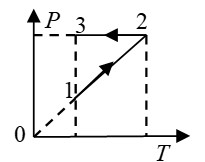
\includegraphics[width=0.3\linewidth]{../figs/VN12-Y24-PH-SYL-014P-9}
	\end{center}
\begin{mcq}(2)
	\item Nung nóng đẳng tích sau đó dãn đẳng áp.
	\item Nung nóng đẳng tích sau đó nén đẳng áp.
	\item Nung nóng đẳng áp sau đó dãn đẳng nhiệt.
	\item Nung nóng đẳng áp sau đó nén đẳng nhiệt.
\end{mcq}
\hideall{
\textbf{Đáp án B.}
}

\item Từ dữ kiện câu trên. Thực hiện quá trình duy nhất nào để từ trạng thái 3 về trạng thái 1?
\begin{mcq}(4)
	\item Nén đẳng nhiệt.
	\item Dãn đẳng nhiệt.
	\item Nén đẳng áp.
	\item Dãn nở đẳng áp.
\end{mcq}
\hideall{
\textbf{Đáp án B.}
}
	
	\item \mkstar{2}\\
	Một lượng khí xác định biến đổi trạng thái (1) sang trạng thái (3) bằng hai đẳng quá trình: đẳng quá trình $(1)\rightarrow(2)$, đẳng quá trình $(2)\rightarrow(3)$ như hình vẽ. Biết nhiệt độ của khí ở trạng thái (1) là $T_1=\SI{200}{\kelvin}$. Nhiệt độ của chất khí ở trạng thái (3) là
	\begin{center}
		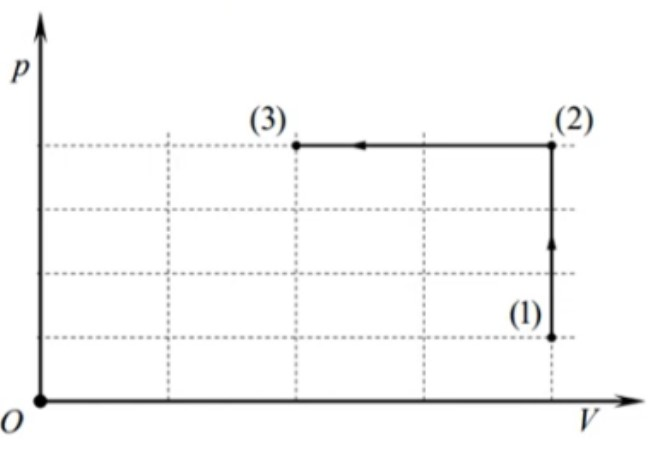
\includegraphics[width=0.45\linewidth]{../figs/VN12-Y24-PH-SYL-014P-1}
	\end{center}
\begin{mcq}(4)
	\item $\SI{200}{\kelvin}$.
	\item $\SI{400}{\kelvin}$.
	\item $\SI{600}{\kelvin}$.
	\item $\SI{300}{\kelvin}$.
\end{mcq}
\hideall{
\textbf{Đáp án B.}\\
\begin{center}
	\begin{tabular}{C{3cm} C{1.5cm}  C{3cm}  C{1.5cm} C{3cm}}
		\colorbox{green!40!white}{\textcolor{red}{\textbf{Trạng thái 1}}} & $\xrightarrow[]{V=const}$ & \colorbox{green!40!white}{\textcolor{red}{\textbf{Trạng thái 2}}} & $\xrightarrow[]{p=const}$ & \colorbox{green!40!white}{\textcolor{red}{\textbf{Trạng thái 3}}}\\
		$T_1=\SI{200}{\kelvin}$ & & $T_2$& & $T_3=?$\\
		$V_1=4$ & & $V_2=4$& & $V_3=2$\\
		$p_1=1$ & & $p_2=4$& & $p_3=4$
	\end{tabular}
\end{center}
Áp dụng phương trình trạng thái khí lí tưởng:
$$\dfrac{p_1V_1}{T_1}=\dfrac{p_3V_3}{T_3}$$
$$\Rightarrow T_3=\SI{400}{\kelvin}.$$
}

\item \mkstar{2}\\
Một lượng khí lí tưởng xác định đã thực hiện quá trình biến đổi trạng thái $(1)-(2)-(3)-(4)$ như hình vẽ. Biết nhiệt độ của chất khí ở trạng thái (1) là $T_1=\SI{600}{\kelvin}$. Nhiệt độ của chất khí này ở trạng thái (4) là
\begin{center}
	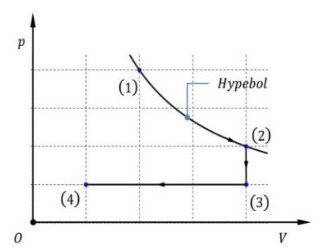
\includegraphics[width=0.45\linewidth]{../figs/VN12-Y24-PH-SYL-014P-3}
\end{center}
\begin{mcq}(4)
	\item $\SI{75}{\kelvin}$.
	\item $\SI{40}{\kelvin}$.
	\item $\SI{60}{\kelvin}$.
	\item $\SI{90}{\kelvin}$.
\end{mcq}
\hideall{
\textbf{Đáp án A.}\\
$$\dfrac{p_1V_1}{T_1}=\dfrac{p_4V_4}{T_4}\Leftrightarrow \dfrac{4\cdot2}{600}=\dfrac{1\cdot1}{T_4}\Rightarrow T_4=\SI{75}{\kelvin}.$$
}

\item \mkstar{2}\\
Cho đồ thị biến đổi trạng thái của một lượng khí lí tưởng từ trạng thái (1) đến trạng thái (2) như hình bên. Tỉ số $T_2/T_1$ là 
\begin{center}
	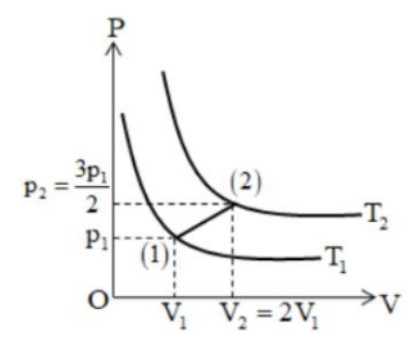
\includegraphics[width=0.45\linewidth]{../figs/VN12-Y24-PH-SYL-014P-2}
\end{center}
\begin{mcq}(4)
	\item 1,5.
	\item 2.
	\item 3. 
	\item 4.
\end{mcq}
\hideall{
\textbf{Đáp án C.}\\
$$\dfrac{p_1V_1}{T_1}=\dfrac{p_2V_2}{T_2}\Rightarrow \dfrac{T_2}{T_1}=\dfrac{p_2V_2}{p_1V_1}=3.$$
}

\item \mkstar{3}\\
Một khí lí tưởng đã thực hiện chu trình biến đổi trạng thái $(1)\rightarrow (2)\rightarrow(3)\rightarrow(4)\rightarrow(1)$ như hình vẽ. Với $(1)\rightarrow(2)$ song song với $(3)\rightarrow(4)$ và song song với $OT$. Biết nhiệt độ của khí tại các trạng thái (1) và (3) lần lượt là $T_1$ và $T_3$. Nhiệt độ của chất khí này tại trạng thái (2) là
\begin{center}
	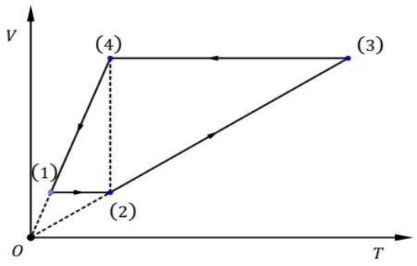
\includegraphics[width=0.45\linewidth]{../figs/VN12-Y24-PH-SYL-014P-4}
\end{center}
\begin{mcq}(4)
	\item $\dfrac{T_1+T_3}{2}$.
	\item $\sqrt{T_1T_3}.$
	\item $\dfrac{T_1-T_3}{2}$.
	\item $\dfrac{T_1T_3}{T_1+T_3}$.
\end{mcq}
\hideall{
\textbf{Đáp án B.}\\
Các quá trình $(4)\rightarrow(1)$ và $(2)\rightarrow(3)$ là đẳng áp:
$$\Rightarrow\begin{cases}
	\dfrac{V_1}{T_1}=\dfrac{V_4}{T_2}\\[8pt]
	\dfrac{V_2}{T_2}=\dfrac{V_3}{T_3}\Leftrightarrow \dfrac{V_1}{T_2}=\dfrac{V_4}{T_3}
\end{cases}
\Rightarrow \dfrac{T_1}{T_2}=\dfrac{T_2}{T_3}\Rightarrow T_2=\sqrt{T_1T_3}.$$
}

\item \mkstar{3}\\
Quá trình giãn nở của một lượng khí lí tưởng khối lượng $m$ ở áp suất $p$ được biểu diễn bằng đường (1) như hình vẽ. Quá trình giãn nở của cùng một loại khí lí tưởng trên, nhưng khối lượng $2m$ và áp suất $2p$ được biểu diễn bằng đường
\begin{center}
	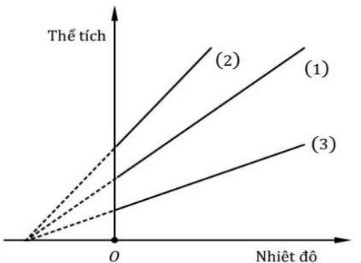
\includegraphics[width=0.35\linewidth]{../figs/VN12-Y24-PH-SYL-014P-5}
\end{center}
\begin{mcq}(2)
	\item (1).
	\item (2).
	\item (3).
	\item Không đáp án nào đúng.
\end{mcq}
\hideall{
\textbf{Đáp án A.}\\
$pV=\dfrac{m}{\mu}RT\Rightarrow V=\dfrac{mR}{p\mu}\cdot T\rightarrow$ nếu cùng tăng $m$ và $p$ lên gấp đôi thì hệ số góc không đổi.
}

\item \mkstar{3}\\
Sự giãn nở của một lượng khí lí tưởng có khối lượng $m$ ở áp suất không đổi $p$ được biểu diễn bằng đường thẳng D. Quá trình giãn nở của cùng một loại khí lí tưởng có khối lượng $2m$ và áp suất $\dfrac{p}{2}$ được thể hiện bởi đường thẳng
\begin{center}
	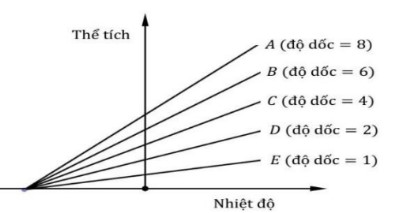
\includegraphics[width=0.45\linewidth]{../figs/VN12-Y24-PH-SYL-014P-6}
\end{center} 
\begin{mcq}(4)
	\item E.
	\item C.
	\item B.
	\item A.
\end{mcq}
\hideall{
\textbf{Đáp án D.}\\
$pV=\dfrac{m}{\mu}RT\Rightarrow V=\dfrac{mR}{p\mu}\cdot T\rightarrow$ nếu tăng $m$ lên 2 lần và giảm $p$ đi 2 lần thì hệ số góc của đường $V\left(T\right)$ tăng 4 lần.
}

\item \mkstar{3}\\
Một mol khí lí tưởng đã thực hiện chu trình biến đổi trạng thái $1-2-3-4-1$ như hình vẽ bên. Trong đó: $V_1=\SI{32}{\liter}$; $T_1=\SI{546}{\kelvin}$; $T_2=\SI{650}{\kelvin}$; $T_3=\SI{1300}{\kelvin}$. Áp suất của khối khí ở trạng thái 3 là
\begin{center}
	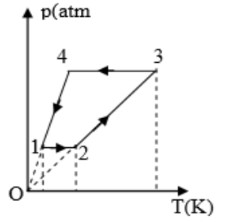
\includegraphics[width=0.35\linewidth]{../figs/VN12-Y24-PH-SYL-014P-7}
\end{center}
\begin{mcq}(4)
	\item $\SI{0.7}{atm}$.
	\item $\SI{2.8}{atm}$.
	\item $\SI{2}{atm}$.
	\item $\SI{1.4}{atm}$.
\end{mcq}
\hideall{
\textbf{Đáp án B.}\\
Qúa trình biến đổi $1-2$ là đẳng áp:
$$\dfrac{V_1}{T_1}=\dfrac{V_2}{T_2}\Rightarrow V_2=\xsi{\dfrac{800}{21}}{\liter}$$
Áp dụng phương trình Clapeyron - Mendeleev:
$$p_3=\dfrac{\nu RT_3}{V_2}\approx\SI{2.8}{atm}.$$
}

\item \mkstar{3}\\
Một mol khí lí tưởng đã thực hiện một chu trình biến đổi trạng thái $1-2-3-4-1$ (hình vẽ). Áp suất $p_1$, $p_2$, $p_3$, $p_4$ lần lượt nhận các giá trị là
\begin{center}
	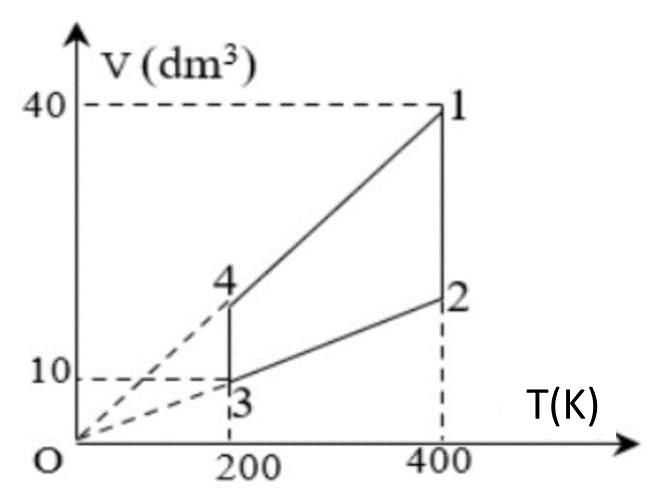
\includegraphics[width=0.35\linewidth]{../figs/VN12-Y24-PH-SYL-014P-8}
\end{center}
\begin{mcq}
	\item $p_1=p_4=\SI{0.83E5}{\pascal}$, $p_2=p_3=\SI{1.66E5}{\pascal}$.
	\item $p_1=p_4=\SI{1.66E5}{\pascal}$, $p_2=p_3=\SI{0.83E5}{\pascal}$.
	\item $p_1=p_4=\SI{0.38E5}{\pascal}$, $p_2=p_3=\SI{6.16E5}{\pascal}$.
	\item $p_1=p_4=\SI{8.3E5}{\pascal}$, $p_2=p_3=\SI{6.6E5}{\pascal}$.
\end{mcq}
\hideall{
\textbf{Đáp án A.}\\
$$p=\dfrac{n RT}{V}\Rightarrow\begin{cases}
	p_1=\dfrac{n RT_1}{V_1}=\SI{83140}{\pascal}\\
	p_2=\dfrac{n RT_2}{V_2}=\SI{166280}{\pascal}
\end{cases}.$$
}
\end{enumerate}

\section{Trắc nghiệm đúng/sai}
\begin{enumerate}[label=\bfseries Câu \arabic*:, leftmargin=1.7cm]
	\item\mkstar{2}\\
 Đồ thị biểu diễn quá trình biến đổi trạng thái của một lượng khí lí tưởng được thể hiện như hình bên.
 \begin{center}
 	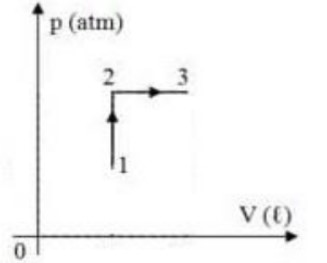
\includegraphics[width=0.35\linewidth]{../figs/VN12-Y24-PH-SYL-014P-15}
 \end{center}
\begin{enumerate}[label=\alph*)]
	\item Từ (1) sang (2) là quá trình đẳng tích.
	\item Từ (2) sang (3) là quá trình đẳng áp.
	\item  Từ (1) sang (2) nhiệt độ khí giảm.
	\item Từ (2) sang (3) nhiệt độ khí giảm.
\end{enumerate}
\hideall{
\begin{enumerate}[label=\alph*)]
	\item Đúng.
	\item Đúng.
	\item Sai.
	\item Sai.
\end{enumerate}
}

\item \mkstar{2}\\
Đồ thị biểu diễn mối liên hệ giữa thể tích khối khí lí tưởng với nhiệt độ được thể hiện như hình bên.
\begin{center}
	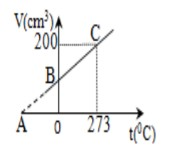
\includegraphics[width=4cm, height=3cm]{../figs/VN12-Y24-PH-SYL-014P-16}
\end{center}
\begin{enumerate}[label=\alph*)]
	\item Trong quá trình biến đổi, áp suất của khối khí không đổi.
	\item Ở trạng thái B khối khí có thể tích $\SI{100}{\centi\meter^3}$.
	\item Khối khí có thể tích bằng $\SI{150}{\centi\meter^3}$ khi nhiệt độ khối khí bằng $\SI{130}{\celsius}$.
	\item Trạng thái A khối khí có nhiệt độ $\SI{-273}{\celsius}$.
\end{enumerate}
\hideall{
\begin{enumerate}[label=\alph*)]
	\item Đúng.
	\item Đúng. 
	$$\dfrac{V_\text{B}}{0+273}=\dfrac{200}{273+273}\Rightarrow V_\text{B}=\SI{100}{\centi\meter^3}.$$
	\item Sai.
	$$\dfrac{150}{130+273}\neq \dfrac{200}{273+273}.$$
	\item Đúng.
\end{enumerate}
}

\item \mkstar{3}\\
Một khối khí lí tưởng ở trạng thái (1) được xác định bởi các thông số $p_1=\SI{1}{atm}$; $V_1=\SI{4}{\liter}$; $T_1=\SI{300}{\kelvin}$. Người ta cho khối khí biến đổi đẳng áp tới trạng thái (2) có nhiệt độ $T_2=\SI{600}{\kelvin}$ và thể tích $V_2$. Cuối cùng, biến đổi đẳng nhiệt tới trạng thái (3) có thể tích $V_3=\SI{2}{\liter}$.
\begin{enumerate}[label=\alph*)]
	\item Áp suất khối khí tại trạng thái (2) là $\SI{2}{atm}$.
	\item Thể tích của khối khí tại trạng thái (2) là $\SI{8}{\liter}$.
	\item Áp suất của khối khí tại trạng thái (3) là $\SI{4}{atm}$.
	\item Trong hệ toạ độ $(p, V)$, đồ thị biểu diễn quá trình biến đổi trạng thái của khối khí từ trạng thái (1) sang trạng thái (2) là một đoạn thẳng đi qua gốc toạ độ, từ trạng thái (2) sang trạng thái (3) là một hyperbol.
\end{enumerate} 
\hideall{
\begin{center}
	\begin{tabular}{|C{3cm}|C{3cm}|C{3cm}|C{3cm}|}
		\hline
		\thead{Trạng thái} & $p$ & $V$ & $T$\\
		\hline
		(1)&$\SI{1}{atm}$ & $\SI{4}{\liter}$ & $\SI{300}{\kelvin}$\\
		\hline
		(2)&$\SI{1}{atm}$ & $V_2$ & $\SI{600}{\kelvin}$\\
		\hline
		(3)&$p_3$ & $\SI{2}{\liter}$ & $\SI{600}{\kelvin}$\\
		\hline
	\end{tabular}
\end{center}
\begin{enumerate}[label=\alph*)]
	\item Sai. $p_2=\SI{1}{atm}$.
	\item Đúng.
	\item Đúng.
	\item Sai. Trong hệ trục toạ độ $\left(p, V\right)$, đồ thị biểu diễn quá trình biến đổi trạng thái của khối khí từ trạng thái (1) sang trạng thái (2) song song với trục $OV$.
\end{enumerate}}

\item \mkstar{3}\\
Một khối khí lí tưởng trong cylanh biến đổi trạng thái qua các giai đoạn như đồ thị hình bên.
\begin{center}
	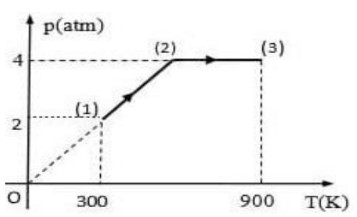
\includegraphics[width=0.45\linewidth]{../figs/VN12-Y24-PH-SYL-014P-17}
\end{center}
\begin{enumerate}[label=\alph*)]
	\item Từ (1) sang (2) là quá trình đẳng tích.
	\item Từ (2) sang (3) là quá trình đẳng áp.
	\item Nhiệt độ ở trạng thái (2) là $\SI{600}{\kelvin}$.
	\item  Nếu thể tích ban đầu ở trạng thái (1) của khối khí là $\SI{12}{\liter}$ thì thể tích của khí ở trạng thái (3) là $\SI{18}{\liter}$.
\end{enumerate}
\hideall{
\begin{center}
	\begin{tabular}{|C{3cm}|C{3cm}|C{3cm}|C{3cm}|}
		\hline
		\thead{Trạng thái} & $p$ & $V$ & $T$\\
		\hline
		(1)&$\SI{2}{atm}$ & $\SI{12}{\liter}$ & $\SI{300}{\kelvin}$\\
		\hline
		(2)&$\SI{4}{atm}$ & $\SI{12}{\liter}$ & $T_2$\\
		\hline
		(3)&$\SI{4}{atm}$ & $V_3$ & $\SI{900}{\kelvin}$\\
		\hline
	\end{tabular}
\end{center}
\begin{enumerate}[label=\alph*)]
	\item Đúng.
	\item Đúng.
	\item Đúng.
	\item Đúng.
\end{enumerate}
}

\end{enumerate}
\section{Bài tập tự luận}
\begin{enumerate}[label=\bfseries Câu \arabic*:, leftmargin=1.7cm]
	\item\mkstar{2}\\
	Cho các đồ thị sau đây biểu diễn chu trình biến đổi trạng thái của các khối khí lí tưởng xác định.
	\begin{center}
		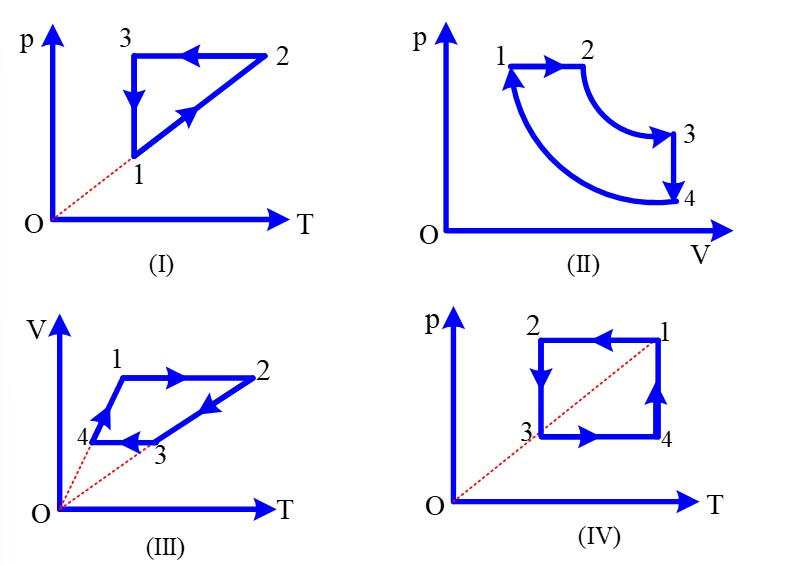
\includegraphics[width=0.65\linewidth]{../figs/VN12-Y24-PH-SYL-014P-10}
	\end{center}
\begin{enumerate}[label=\alph*)]
	\item Vẽ lại đồ thị (I) trong các hệ toạ độ $\left(V, T\right)$, $\left(p, V\right)$.
	\item Vẽ lại đồ thị (II) trong các hệ toạ độ  $\left(V,T\right)$, $\left(p, T\right)$.
	\item Vẽ lại đồ thị (III) trong các hệ toạ độ $\left(p, V\right)$, $\left(p, T\right)$.
	\item Vẽ lại đồ thị (IV) trong các hệ toạ độ $\left(p, V\right)$, $\left(V, T\right)$.
\end{enumerate}
\hideall{
\begin{enumerate}[label=\alph*)]
	\item (1) đến (2) là quá trình đẳng tích, $p$ tăng, $T$ tăng.\\
	(2) đến (3) là quá trình đẳng áp, $T$ giảm, $V$ giảm.\\
	(3) đến (1) là quá trình đẳng nhiệt, $p$ giảm, $V$ tăng.
	\begin{center}
		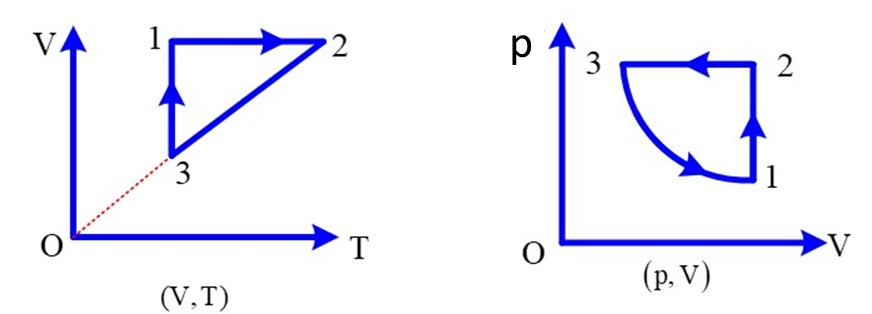
\includegraphics[width=0.65\linewidth]{../figs/VN12-Y24-PH-SYL-014P-11}
	\end{center}
\item (1) đến (2) là quá trình đẳng áp, $V$ tăng, $T$ tăng.\\
(2) đến (3) là quá trình đẳng nhiệt, $p$ giảm, $V$ tăng.\\
(3) đến (4) là quá trình đẳng tích, $p$ giảm, $T$ giảm.\\
(4) đến (1) là quá trình đẳng nhiệt, $p$ tăng, $V$ giảm.
\begin{center}
	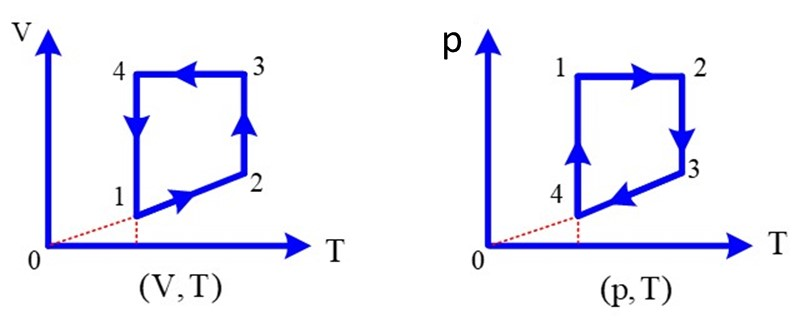
\includegraphics[width=0.65\linewidth]{../figs/VN12-Y24-PH-SYL-014P-12}
\end{center} 
\item (1) đến (2) là quá trình đẳng tích, $T$ tăng, $p$ tăng.\\
(2) đến (3) là quá trình đẳng áp, $T$ giảm, $V$ giảm.\\
(3) đến (4) là quá trình đẳng tích, $T$ giảm, $p$ giảm.\\
(4) đến (1) là quá trình đẳng áp, $T$ tăng, $V$ tăng.
\begin{center}
	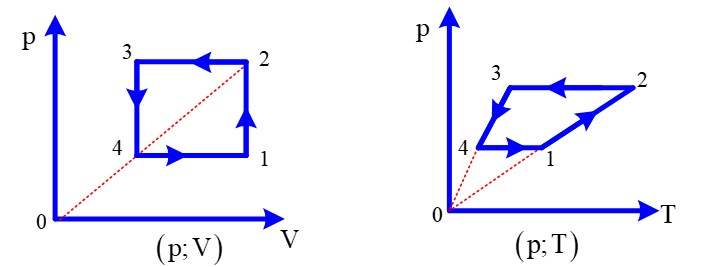
\includegraphics[width=0.65\linewidth]{../figs/VN12-Y24-PH-SYL-014P-13}
\end{center}
\item (1) đến (2) là quá trình đẳng áp, $T$ giảm, $V$ giảm.\\
(2) đến (3) là quá trình đẳng nhiệt, $p$ giảm, $V$ tăng.\\
(3) đến (4) là quá trình đẳng áp, $T$ tăng, $V$ tăng.\\
(4) đến (1) là quá trình đẳng nhiệt, $p$ tăng, $V$ giảm.
\begin{center}
	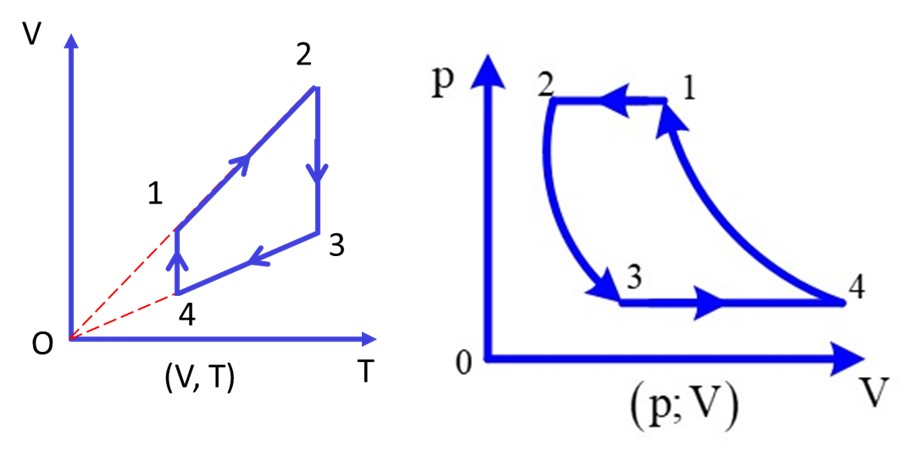
\includegraphics[width=0.65\linewidth]{../figs/VN12-Y24-PH-SYL-014P-14.jpg}
\end{center}
\end{enumerate}
}

\item \mkstar{3}\\
Một lượng khí oxygen ở nhiệt độ $\SI{130}{\celsius}$ dưới áp suất $\SI{E5}{\newton/\meter^2}$ được nén đẳng nhiệt đến áp suất $\SI{1.3E5}{\newton/\meter^2}$. Cần làm lạnh đẳng tích đến nhiệt độ nào để áp suất khí giảm bằng lúc đầu?\\
Biểu diễn quá trình biến đổi trên trong các hệ toạ độ $\left(p, V\right)$, $\left(p, T\right)$, $\left(V, T\right)$.
\hideall{
\begin{center}
	\begin{tabular}{C{3cm} C{1.5cm}  C{3cm}  C{1.5cm} C{3cm}}
		\colorbox{green!40!white}{\textcolor{red}{\textbf{Trạng thái 1}}} & $\xrightarrow[]{T=const}$ & \colorbox{green!40!white}{\textcolor{red}{\textbf{Trạng thái 2}}} & $\xrightarrow[]{V=const}$ & \colorbox{green!40!white}{\textcolor{red}{\textbf{Trạng thái 3}}}\\
		$T_1=\SI{403}{\kelvin}$ & & $T_2=\SI{403}{\kelvin}$& & $T_3=?$\\
		$p_1=\SI{E5}{\newton/\meter^2}$ & & $p_2=\SI{1.3E5}{\newton/\meter^2}$& & $p_3=\SI{E5}{\newton/\meter^2}$
	\end{tabular}
\end{center}
Áp dụng định luật Charles cho quá trình biến đổi $(2)\rightarrow(3)$:
$$\dfrac{p_3}{T_3}=\dfrac{p_2}{T_2}\Rightarrow T_3=\dfrac{p_2T_2}{p_3}=\SI{310}{\kelvin}\rightarrow t_3=\SI{37}{\celsius}.$$
Đồ thị biểu diễn quá trình biến đổi trạng thái của khối khí trong các hệ trục toạ độ:\\
\begin{center}
	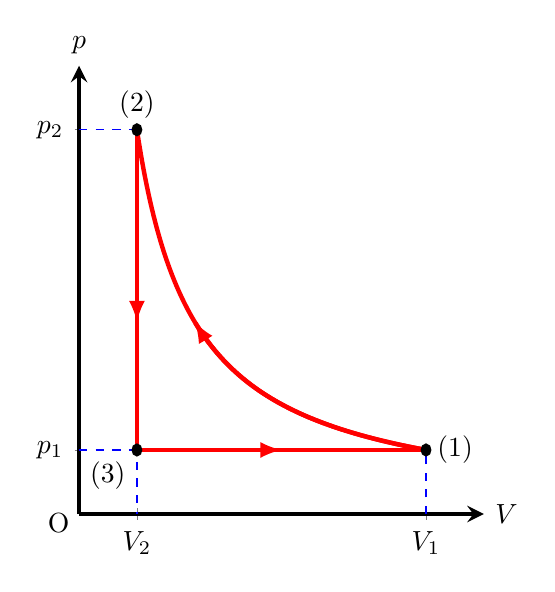
\begin{tikzpicture}  
		\begin{axis}[  ultra thick,xscale=0.75,
			xmin=0,  
			xmax=7,  
			ytick={1,6},
			xtick={1,6},
			ymin=0,  
			ymax=7, 
			samples=300,
			yticklabels={$p_1$, $p_2$},
			xticklabels={$V_2$, $V_1$},
			axis lines=center, 
			xlabel=$V$, 
			ylabel=$p$, 
			every axis y label/.style={at=(current axis.above origin),anchor=south},  
			every axis x label/.style={at=(current axis.right of origin),anchor=west},  ]
			\draw[line width=0.5pt,blue, dashed] (axis cs: 0, 6) -- (axis cs: 1, 6);
			\draw[line width=0.5pt,blue, dashed] (axis cs: 0, 1) -- (axis cs: 1, 1);
			\draw[line width=0.5pt,blue, dashed] (axis cs: 6, 0) -- (axis cs: 6, 1);
			\draw[line width=0.5pt,blue, dashed] (axis cs: 1, 6) -- (axis cs: 1, 0);
			\draw[ultra thick, red] (axis cs: 1, 6) -- (axis cs:1, 1);
			\draw[ultra thick,-latex, red] (axis cs: 1, 6) -- (axis cs: 1, 3);
			\addplot [ultra thick, red, smooth, domain=1:6] {6/x};   
			\addplot [ultra thick,-latex,red, smooth, domain=6:2] {6/x} ; 
			\addplot [ultra thick, red, smooth, domain=1:6] {1}; 
			\addplot [ultra thick,-latex, red, smooth, domain=1:3.5] {1};
			\filldraw[black] (axis cs:6,1) circle (1.5pt) node[right] {(1)};
			\filldraw[black] (axis cs:1,6) circle (1.5pt) node[above] {(2)};
			\filldraw[black] (axis cs:1,1) circle (1.5pt) node[below left] {(3)};
		\end{axis}  
		\node[label={[below left]90:O}] at (0,0){};
	\end{tikzpicture}
\end{center}
\begin{minipage}{0.5\textwidth}
	\begin{center}
		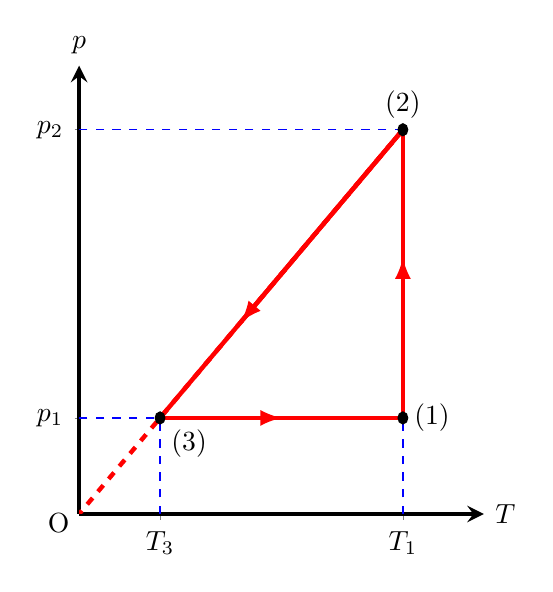
\begin{tikzpicture}  
			\begin{axis}[  ultra thick,xscale=0.75,
				xmin=0,  
				xmax=5,  
				ytick={0.75,3},
				xtick={1,4},
				ymin=0,  
				ymax=3.5, 
				samples=300,
				yticklabels={$p_1$, $p_2$},
				xticklabels={$T_3$, $T_1$},
				axis lines=center, 
				xlabel=$T$, 
				ylabel=$p$, 
				every axis y label/.style={at=(current axis.above origin),anchor=south},  
				every axis x label/.style={at=(current axis.right of origin),anchor=west},  ]
				\draw[line width=0.5pt,blue, dashed] (axis cs: 4, 0.75) -- (axis cs: 0, 0.75);
				\draw[line width=0.5pt,blue, dashed] (axis cs: 4, 3) -- (axis cs: 0, 3);
				\draw[line width=0.5pt,blue, dashed] (axis cs: 4, 0) -- (axis cs: 4, 0.75);
				\draw[line width=0.5pt,blue, dashed] (axis cs: 1, 0) -- (axis cs: 1, 0.75);
				\draw[ultra thick, red] (axis cs: 4, 0.75) -- (axis cs: 4, 3);
				\draw[ultra thick,-latex, red] (axis cs: 4, 0.75) -- (axis cs: 4, 2);
				\addplot [ultra thick, red, dashed, smooth, domain=4:0] {0.75*x};
				\addplot [ultra thick, red, smooth, domain=4:1] {0.75*x};  
				\addplot [ultra thick,-latex,red, smooth, domain=4:2] {0.75*x} ; 
				\addplot [ultra thick, red, smooth, domain=1:4] {0.75};  
				\addplot [ultra thick,-latex,red, smooth, domain=1:2.5] {0.75} ;

				\filldraw[black] (axis cs:4,0.75) circle (1.5pt) node[right] {(1)};
				\filldraw[black] (axis cs:4,3) circle (1.5pt) node[above] {(2)};
				\filldraw[black] (axis cs:1,0.75) circle (1.5pt) node[below right] {(3)};
			\end{axis}  
			\node[label={[below left]90:O}] at (0,0){};
		\end{tikzpicture}
	\end{center}
\end{minipage}\hfill
\begin{minipage}{0.5\textwidth}
	\begin{center}
		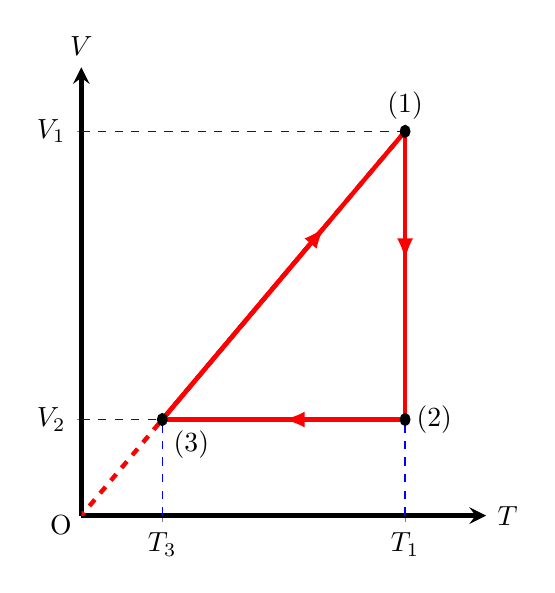
\begin{tikzpicture}  
			\begin{axis}[  ultra thick,xscale=0.75,
				xmin=0,  
				xmax=5,  
				ytick={0.75,3},
				xtick={1,4},
				ymin=0,  
				ymax=3.5, 
				samples=300,
				yticklabels={$V_2$, $V_1$},
				xticklabels={$T_3$, $T_1$},
				axis lines=center, 
				xlabel=$T$, 
				ylabel=$V$, 
				every axis y label/.style={at=(current axis.above origin),anchor=south},  
				every axis x label/.style={at=(current axis.right of origin),anchor=west},  ]
				\draw[line width=0.5pt,blue, dashed] (axis cs: 4, 0.75) -- (axis cs: 0, 0.75);
				\draw[line width=0.5pt,blue, dashed] (axis cs: 4, 3) -- (axis cs: 0, 3);
				\draw[line width=0.5pt,blue, dashed] (axis cs: 4, 0) -- (axis cs: 4, 0.75);
				\draw[line width=0.5pt,blue, dashed] (axis cs: 1, 0) -- (axis cs: 1, 0.75);
				\draw[ultra thick, red] (axis cs: 4, 0.75) -- (axis cs: 4, 3);
				\draw[ultra thick,-latex, red] (axis cs: 4, 3) -- (axis cs: 4, 2);
				\addplot [ultra thick, red, dashed, smooth, domain=4:0] {0.75*x};
				\addplot [ultra thick, red, smooth, domain=4:1] {0.75*x};  
				\addplot [ultra thick,-latex,red, smooth, domain=1:3] {0.75*x} ; 
				\addplot [ultra thick, red, smooth, domain=1:4] {0.75};  
				\addplot [ultra thick,-latex,red, smooth, domain=4:2.5] {0.75} ;
				
				\filldraw[black] (axis cs:4,0.75) circle (1.5pt) node[right] {(2)};
				\filldraw[black] (axis cs:4,3) circle (1.5pt) node[above] {(1)};
				\filldraw[black] (axis cs:1,0.75) circle (1.5pt) node[below right] {(3)};
			\end{axis}  
			\node[label={[below left]90:O}] at (0,0){};
		\end{tikzpicture}
	\end{center}
\end{minipage}

}

\item \mkstar{3}\\
Một khối lượng $m=\SI{1}{\gram}$ khí helium trong cylanh, ban đầu có thể tích $V_1=\SI{4.2}{\liter}$, nhiệt độ $t_1=\SI{27}{\celsius}$. Khí biến đổi trạng thái theo một chu trình kín gồm ba giai đoạn:
\begin{itemize}
	\item \textit{Giai đoạn 1:} Giãn nở đẳng áp, thể tích tăng lên đến $\SI{6.3}{\liter}$.
	\item \textit{Giai đoạn 2:} Nén đẳng nhiệt.
	\item \textit{Giai đoạn 3:} Làm lạnh đẳng tích.
\end{itemize}
\begin{enumerate}[label=\alph*)]
	\item Vẽ đồ thị biểu diễn chu trình trong các hệ toạ độ $\left(p, V\right)$, $\left(V, T\right)$, $\left(p, T\right)$.
	\item Tìm nhiệt độ và áp suất tính theo đơn vị $\si{at}$ lớn nhất đạt được trong chu trình.
\end{enumerate}
\hideall{
\begin{enumerate}[label=\alph*)]
	\item Đồ thị biểu diễn chu trình biến đổi trạng thái:
\begin{center}
	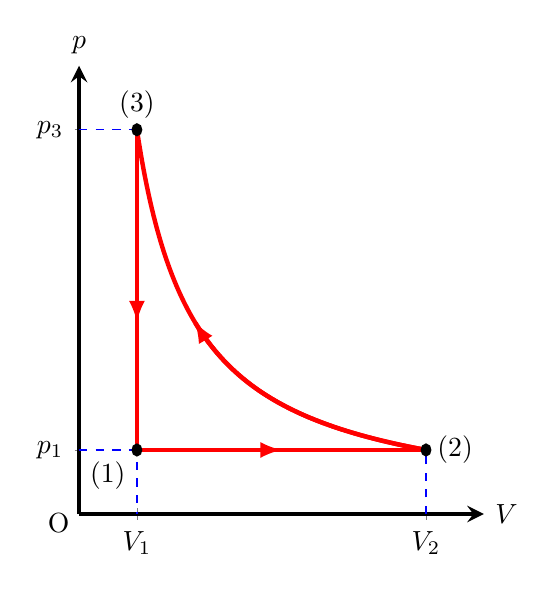
\begin{tikzpicture}  
		\begin{axis}[  ultra thick,xscale=0.75,
			xmin=0,  
			xmax=7,  
			ytick={1,6},
			xtick={1,6},
			ymin=0,  
			ymax=7, 
			samples=300,
			yticklabels={$p_1$, $p_3$},
			xticklabels={$V_1$, $V_2$},
			axis lines=center, 
			xlabel=$V$, 
			ylabel=$p$, 
			every axis y label/.style={at=(current axis.above origin),anchor=south},  
			every axis x label/.style={at=(current axis.right of origin),anchor=west},  ]
			\draw[line width=0.5pt,blue, dashed] (axis cs: 0, 6) -- (axis cs: 1, 6);
			\draw[line width=0.5pt,blue, dashed] (axis cs: 0, 1) -- (axis cs: 1, 1);
			\draw[line width=0.5pt,blue, dashed] (axis cs: 6, 0) -- (axis cs: 6, 1);
			\draw[line width=0.5pt,blue, dashed] (axis cs: 1, 6) -- (axis cs: 1, 0);
			\draw[ultra thick, red] (axis cs: 1, 6) -- (axis cs:1, 1);
			\draw[ultra thick,-latex, red] (axis cs: 1, 6) -- (axis cs: 1, 3);
			\addplot [ultra thick, red, smooth, domain=1:6] {6/x};   
			\addplot [ultra thick,-latex,red, smooth, domain=6:2] {6/x} ; 
			\addplot [ultra thick, red, smooth, domain=1:6] {1}; 
			\addplot [ultra thick,-latex, red, smooth, domain=1:3.5] {1};
			\filldraw[black] (axis cs:6,1) circle (1.5pt) node[right] {(2)};
			\filldraw[black] (axis cs:1,6) circle (1.5pt) node[above] {(3)};
			\filldraw[black] (axis cs:1,1) circle (1.5pt) node[below left] {(1)};
		\end{axis}  
		\node[label={[below left]90:O}] at (0,0){};
	\end{tikzpicture}
\end{center}
\begin{minipage}{0.5\textwidth}
	\begin{center}
		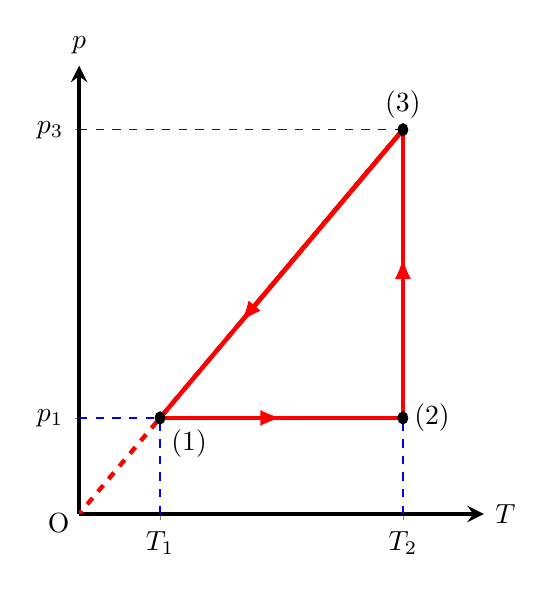
\begin{tikzpicture}  
			\begin{axis}[  ultra thick,xscale=0.75,
				xmin=0,  
				xmax=5,  
				ytick={0.75,3},
				xtick={1,4},
				ymin=0,  
				ymax=3.5, 
				samples=300,
				yticklabels={$p_1$, $p_3$},
				xticklabels={$T_1$, $T_2$},
				axis lines=center, 
				xlabel=$T$, 
				ylabel=$p$, 
				every axis y label/.style={at=(current axis.above origin),anchor=south},  
				every axis x label/.style={at=(current axis.right of origin),anchor=west},  ]
				\draw[line width=0.5pt,blue, dashed] (axis cs: 4, 0.75) -- (axis cs: 0, 0.75);
				\draw[line width=0.5pt,blue, dashed] (axis cs: 4, 3) -- (axis cs: 0, 3);
				\draw[line width=0.5pt,blue, dashed] (axis cs: 4, 0) -- (axis cs: 4, 0.75);
				\draw[line width=0.5pt,blue, dashed] (axis cs: 1, 0) -- (axis cs: 1, 0.75);
				\draw[ultra thick, red] (axis cs: 4, 0.75) -- (axis cs: 4, 3);
				\draw[ultra thick,-latex, red] (axis cs: 4, 0.75) -- (axis cs: 4, 2);
				\addplot [ultra thick, red, dashed, smooth, domain=4:0] {0.75*x};
				\addplot [ultra thick, red, smooth, domain=4:1] {0.75*x};  
				\addplot [ultra thick,-latex,red, smooth, domain=4:2] {0.75*x} ; 
				\addplot [ultra thick, red, smooth, domain=1:4] {0.75};  
				\addplot [ultra thick,-latex,red, smooth, domain=1:2.5] {0.75} ;
				
				\filldraw[black] (axis cs:4,0.75) circle (1.5pt) node[right] {(2)};
				\filldraw[black] (axis cs:4,3) circle (1.5pt) node[above] {(3)};
				\filldraw[black] (axis cs:1,0.75) circle (1.5pt) node[below right] {(1)};
			\end{axis}  
			\node[label={[below left]90:O}] at (0,0){};
		\end{tikzpicture}
	\end{center}
\end{minipage}\hfill
\begin{minipage}{0.5\textwidth}
	\begin{center}
		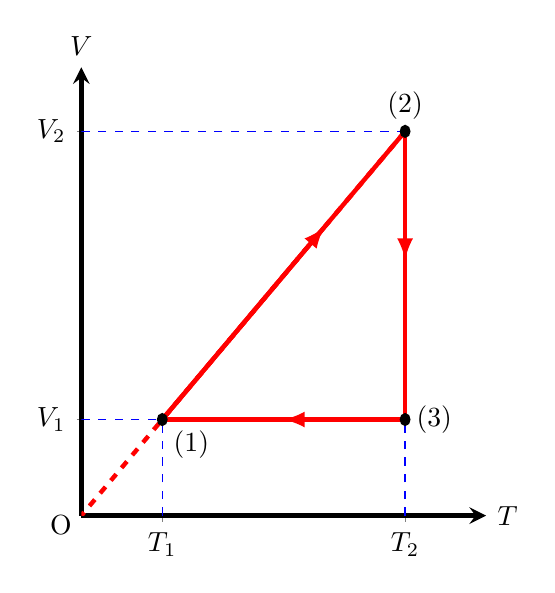
\begin{tikzpicture}  
			\begin{axis}[  ultra thick,xscale=0.75,
				xmin=0,  
				xmax=5,  
				ytick={0.75,3},
				xtick={1,4},
				ymin=0,  
				ymax=3.5, 
				samples=300,
				yticklabels={$V_1$, $V_2$},
				xticklabels={$T_1$, $T_2$},
				axis lines=center, 
				xlabel=$T$, 
				ylabel=$V$, 
				every axis y label/.style={at=(current axis.above origin),anchor=south},  
				every axis x label/.style={at=(current axis.right of origin),anchor=west},  ]
				\draw[line width=0.5pt,blue, dashed] (axis cs: 4, 0.75) -- (axis cs: 0, 0.75);
				\draw[line width=0.5pt,blue, dashed] (axis cs: 4, 3) -- (axis cs: 0, 3);
				\draw[line width=0.5pt,blue, dashed] (axis cs: 4, 0) -- (axis cs: 4, 0.75);
				\draw[line width=0.5pt,blue, dashed] (axis cs: 1, 0) -- (axis cs: 1, 0.75);
				\draw[ultra thick, red] (axis cs: 4, 0.75) -- (axis cs: 4, 3);
				\draw[ultra thick,-latex, red] (axis cs: 4, 3) -- (axis cs: 4, 2);
				\addplot [ultra thick, red, dashed, smooth, domain=4:0] {0.75*x};
				\addplot [ultra thick, red, smooth, domain=4:1] {0.75*x};  
				\addplot [ultra thick,-latex,red, smooth, domain=1:3] {0.75*x} ; 
				\addplot [ultra thick, red, smooth, domain=1:4] {0.75};  
				\addplot [ultra thick,-latex,red, smooth, domain=4:2.5] {0.75} ;
				
				\filldraw[black] (axis cs:4,0.75) circle (1.5pt) node[right] {(3)};
				\filldraw[black] (axis cs:4,3) circle (1.5pt) node[above] {(2)};
				\filldraw[black] (axis cs:1,0.75) circle (1.5pt) node[below right] {(1)};
			\end{axis}  
			\node[label={[below left]90:O}] at (0,0){};
		\end{tikzpicture}
	\end{center}
\end{minipage}
\item Quá trình (1)-(2) là đẳng áp nên:
$$\dfrac{V_1}{T_1}=\dfrac{V_2}{T_2}\Rightarrow T_2=\dfrac{V_2}{V_1}T_1=\SI{450}{\kelvin}.$$
Quá trình (2)-(3) là đẳng nhiệt nên:
$$T_3=T_2=\SI{450}{\kelvin}.$$
Áp suất ở trạng thái (3):
$$p_3=\dfrac{n RT_3}{V_3}\approx\SI{222589.29}{\pascal}=\SI{2.27}{at}.$$
Vậy $T_\text{max}=T_2=\SI{450}{\kelvin}$ và $p_\text{max}=p_3=\SI{2.27}{at}.$
\end{enumerate}
}

\item \mkstar{4}\\
Có $\SI{20}{\gram}$ khí helium chứa trong cylanh đậy kín bởi piston  biến đổi chậm từ $(1)\rightarrow(2)$ theo đồ thị mô tả bởi hình bên.
\begin{center}
	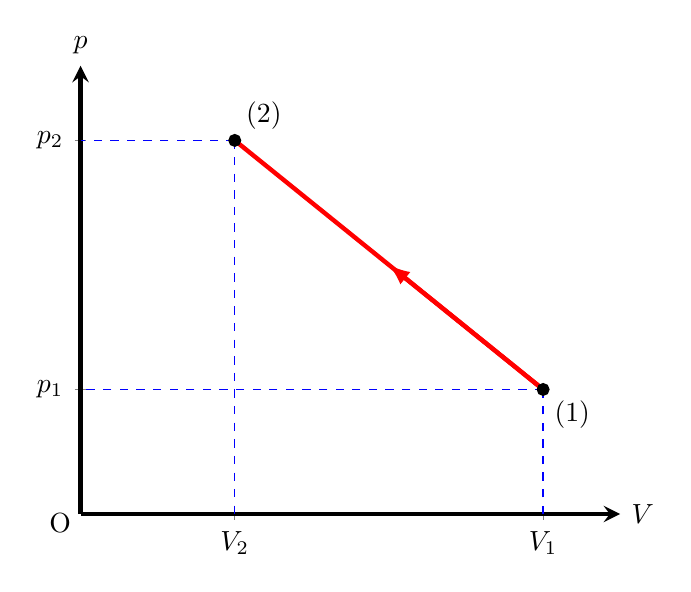
\begin{tikzpicture}  
		\begin{axis}[  ultra thick,
			xmin=0,  
			xmax=35,  
			ytick={5,15},
			xtick={10,30},
			ymin=0,  
			ymax=18, 
			samples=300,
			yticklabels={$p_1$, $p_2$},
			xticklabels={$V_2$, $V_1$},
			axis lines=center, 
			xlabel=$V$, 
			ylabel=$p$, 
			every axis y label/.style={at=(current axis.above origin),anchor=south},  
			every axis x label/.style={at=(current axis.right of origin),anchor=west},  ]
			\draw[line width=0.5pt,blue, dashed] (axis cs: 10, 15) -- (axis cs: 10, 0);
			\draw[line width=0.5pt,blue, dashed] (axis cs: 10, 15) -- (axis cs: 0, 15);
			\draw[line width=0.5pt,blue, dashed] (axis cs: 30, 0) -- (axis cs: 30, 5);
			\draw[line width=0.5pt,blue, dashed] (axis cs: 30, 5) -- (axis cs: 0, 5);
			\draw[ultra thick, red] (axis cs: 30, 5) -- (axis cs: 10, 15);
			\draw[ultra thick,-latex, red] (axis cs: 30, 5) -- (axis cs: 20, 10);
			\filldraw[black] (axis cs:30,5) circle (1.5pt) node[below right] {(1)};
			\filldraw[black] (axis cs:10,15) circle (1.5pt) node[above right] {(2)};
		\end{axis}  
		\node[label={[below left]90:O}] at (0,0){};
	\end{tikzpicture}
\end{center}
Cho: $V_1=\SI{30}{\liter}$; $p_1=\SI{5}{atm}$; $V_2=\SI{10}{\liter}$; $p_2=\SI{15}{atm}$. Hãy tìm nhiệt độ cao nhất mà khí đạt được trong quá trình biến đổi trạng thái.
\hideall{
Quá trình biến đổi trạng thái từ $(1)\rightarrow (2)$ có dạng:
$$p=aV+b$$
Ta có:
$$\begin{cases}
	V_1=\SI{30}{\liter}\Leftrightarrow p_1=\SI{5}{atm}\\
	V_2=\SI{10}{\liter}\Leftrightarrow p_2=\SI{15}{atm}
\end{cases}\Leftrightarrow \begin{cases}
30a+b=5\\
10a+b=15
\end{cases}\Rightarrow \begin{cases}
a=\SI{-0.5}{atm/\liter}\\
b=\SI{20}{atm}
\end{cases}.$$
Như vậy:
\begin{equation}
	\label{eq:14P-1}\\
	p=-0,5V+20
\end{equation}
Theo phương trình Clapeyron - Mendeleev:
\begin{equation}
	\label{eq:14P-2}\\
	pV=n RT
\end{equation}
Từ (\ref{eq:14P-1}) và (\ref{eq:14P-2}), ta thu được:
$$T=\dfrac{1}{n R}\left(-0,5V^2+20V\right).$$
Khối khí đạt nhiệt độ cực đại khi $V=\SI{20}{\liter}$:
$$T_\text{max}=\dfrac{M}{mR}\left(-0,5V^2+20V\right)=\dfrac{\left(\SI{4}{\gram/\mole}\right)}{\left(\SI{20}{\gram}\right)\cdot\left(\SI{0.082}{\dfrac{atm\cdot\liter}{\mole\cdot\kelvin}}\right)}\cdot\left[\left(-\SI{0.5}{atm/\liter}\right)\cdot\left(\SI{20}{\liter}\right)^2+\left(\SI{20}{atm}\right)\cdot\left(\SI{20}{\liter}\right)\right]\approx\SI{487.8}{\kelvin}.$$
}
\end{enumerate}






